% Capitulo 2
\chapter{The Problem}\label{theProblemChap}
In this section we detail the problem that we tackle in this study. A good understanding of the previous sections and of the systematic mapping available in \cite{fabioMartinSM} is required.

\section{Problem Breakdown}

For a long time the industry developed applications storing data on relational databases. Graph databases, Search Engines, Document stores, Wide Column Store and other types of database systems emerged over the last years as a demand of the industry. 

New categories and types of database systems are capable of processing and accessing data in new ways that relational DBs do not support. In other words, for some application, using relational databases may not be the best fit. 

When developing an application, it is not always possible to use the technology that is most suited to the application use cases and requirements. This situation is due to a number of reasons. In an Agile project, for example, not always the team knows all use-cases and application requirements at once, as the Agile Manifesto states: ``Welcome changing requirements, even late in 
development. Agile processes harness change for 
the customer's competitive advantage.'' \cite{fowler2001agile}. 

Furthermore, using several databases on the early releases of a software product may add unnecessary complexity to the code base and might become an overengineering problem over time. 

The fact that some applications are built not knowing beforehand all the requirements, use-cases and expected workload on production environments - \textit{(\textbf{how much} will it scale?}) - often leads to database transitioning scenarios.

In fact, applications that work with more than one database type are popular at the present time, as \cite{sadalage2012nosql} reveals. Some companies, as Instaclustr \cite{instaclustr} and \cite{elastic}, emerged in order to provide support and consultancy to database transitioning scenarios.

There are other cases, also, where an application is developed using an existing database technology, as MySQL, and a number of improvements are made on it, leading to the rise of new databases. Twitter FlockDB \cite{flockdb}, a distributed \& fault-tolerant graph database, emerged in these conditions. 


\subsection{Database transitions in the industry}

Database transitioning processes are not easy and straightforward tasks depending on the size of the application. A number of steps is required when performing database transitions, as revealed on Section~\ref{introductionChap}.

On the other side, a structured process is not always followed when transitioning migrating databases on production environments. \cite{fabioMartinSM} revealed, for instance, that database transition scenarios on the industry follow non-standardized methods and that they may vary significantly among applications. This situation may lead to losses, rework and a hard to maintain codebase.

There are some industry reports, as the ones from Coursera, a leading Education Technology company with over 10 million users \cite{courserawiki}, where more than one database transitions were made in a brief period of time.  

Frank Chen, member of Coursera's engineering team, enlightened the reasons why Coursera replaced part of its database technology from MongoDB (NoSQL DB) to MySQL(Relational DB) \cite{coursera-mongodb-mysql} . 

In other post \cite{coursera-mongodb-mysql2}, Chen also reveals that part of the MySQL architecture was migrated in a second step to Cassandra (NoSQL DB). A blog post from Coursera's Engineering team confirms and discusses more about the transition from MySQL to Cassandra \cite{coursera-mysql-cassandra}. 

Analyzing all the conditions evidenced on this section, a problem to our study was defined: How can a database transition be made in a pragmatic manner? What are the steps and pitfalls to be avoided in relational to NoSQL transitions? 

\section{Proposed solution}

In this work we propose a set of steps to guide the transition from relational databases to NoSQL ones. The suggested guidelines make use of a set of Service Level Agreements (SLAs) to guide the whole process. These guidelines are represented on Figure~\ref{fig:guidelinesNoSQL}.

When an application or website grows, a good strategy is to isolate the application server and database server in two distinct machines, as \cite{dorm} suggests.

If a machine shares its resources among Web Servers, DB Servers and other applications, for example, a high CPU load on the web server side may impact the performance of the Database, downgrading its performance. The guidelines proposed in this work assume that the database server is isolated on its own machine.

\begin{figure}[ht!]
\centering
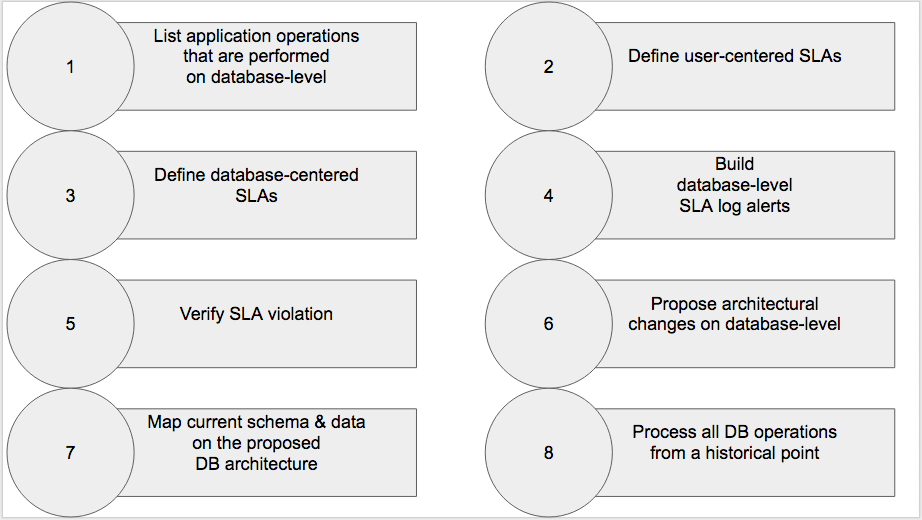
\includegraphics[width=150mm]{Imagens/guidelines.png}
\caption{Relational to NoSQL Steps.\label{fig:guidelinesNoSQL}}
\end{figure}

\subsection{List application operations that are performed on database-level}

A database transition can be motivated by a number of reasons, as budget, lack of support from the community and performance issues. Migrations scenarios motivated by performance issues are the focus of this study, as other reasons might be very specific to each application / transition scenario. 

Performance issues might be caused by database growth or by new application requirements. The first step in a transition scenario is, then, to identify \textit{which} are the application operations or requirements that are driving the transition. 

To identify these operations, it is necessary to explicitly enumerate the application operations that are performed on database level. To illustrate the process of enumerating these operations, consider the following application examples: 

\textbf{A retail business-intelligence application: } A retail business-intelligence application can be used by large retail corporations and supermarket chains. Some use-cases that perform database-level operations on this kind of applications may be:

\begin{itemize}
\item{To process consumer purchases;}
\item{To clusterize customers by their consumption profiles;}
\item{To export summarized reports of transactions that happened last week;}
\end{itemize}

\textbf{Social Networks:} A social network is a category of applications where users generally may befriend / follow other users, publish posts and share their own content. On this kind of applications. Some use-cases that perform database-level operations are: 

\begin{itemize}
\item{Follow or befriend another user;}
\item{Publis posts;}
\item{List user timeline;}
\end{itemize}


\subsection{Define user-centered SLAs}

For each database operation enumerated on the previous step, a \textbf{user-centered} wheighted-partial SLA is defined with the stakeholders of the application. For these SLAs, two thresholds must be explicitly defined for each operation: an \textbf{``ideal threshold''} and a \textbf{``tolerable threshold''}.

\textbf{\textit{Ideal threshold}} is the performance level that is expected by application users. The \textbf{\textit{tolerable threshold}} is a threshold where users can still use the application but the user experience with the application is downgraded.

When the \textbf{\textit{tolerable threshold}} is broken, user experience is dramatically affected and (part of) the application may not be operational for its users.

An example of user-centered SLA is given in the context of the retail business-intelligence application previously defined to illustrate this concept: 

\begin{itemize}
\item{ 
\textbf{Process consumer purchase (Store credit card transaction on my Data Warehouse}
\subitem{\textbf{Ideal Threshold:} up to 1 seconds;}
\subitem{\textbf{Tolerable threshold:} up to 1 minute;}
}

In other words, the user expects a purchase to be processed in one second. If it takes up to 60 seconds, the application can still be used, despite it may affect user's experience. If a purchase takes more than 60 seconds to be processed, users may get really frustrated and long lines may be expected on the cashier.

\item{
\textbf{Export summarized report of transactions that happened last week (Retrieve and perform aggregation operations on selected records) }
\subitem{\textbf{Ideal Threshold:} up to 24 hours;}
\subitem{\textbf{Tolerable threshold:} up to 72 hours;}
}
\end{itemize}
     
In other words, the app user expects that a summarized report of last week's transactions is made available in up to 24 hours. If the exported report takes more than 3 days (72h) to be generated, the application is not useful to the user anymore, as the business strategy might be severely affected by application performance.

The \textbf{\textit{SLA Delta}} between the \textbf{\textit{Ideal Threshold}} and \textbf{\textit{Tolerable Threshold}} is defined as the number of \textbf{\textit{Ideal SLAs}} that can fit inside \textbf{\textit{Tolerable SLA}}. From this concept, we can define the \textbf{\textit{SLA Delta}} for the operations defined above:

\begin{itemize}
\item{ 
\textbf{Process consumer purchase (Store credit card transaction on my Data Warehouse)}
\subitem{\textbf{Ideal Threshold:} up to 1 seconds;}
\subitem{\textbf{Tolerable threshold:} up to 1 minute;}
\subitem{\textbf{SLA Delta:} 6.000\% (60x)}
}

\item{
\textbf{Export summarized report of transactions that happened last week (Retrieve and perform aggregation operations on selected records) }
\subitem{\textbf{Ideal Threshold:} up to 24 hours;}
\subitem{\textbf{Tolerable threshold:} up to 72 hours;}
\subitem{\textbf{SLA Delta:} 300\% (3x)}
}

\end{itemize}

The \textbf{SLA delta} is always equals to or greater than 100\% by definition, and will be used as a parameter on the following steps of the proposed guidelines.

As stated previously, the \textbf{ideal threshold} and \textbf{tolerable threshold} should be defined with the application stakeholders as quantifiable metrics. The \textbf{SLA Delta} can be obtained as the division: \textbf{tolerable threshold} / \textbf{ideal threshold}.

As we will be targeting performance issues at database level, \textbf{ideal threshold}, \textbf{tolerable threshold} and \textbf{SLA delta} can generally be seen as a time-related metrics, as it is shown on the examples above. 

In fact, \textit{time} is the main metric when benchmarking databases, as presented on \cite{datastaxbenchmark} - operations/sec and latency. Other quantifiable metrics and Key Performance Indicators (KPIs), as \textit{processed workload} and \textit{client CPU / memory usage} can also be used as metrics to the thresholds, however. I.E: it is also possible to define thresholds related to the client CPU usage, for example. 

On Figure~\ref{fig:thresholds} it is possible to graphically visualize the concepts of \textbf{Ideal Threshold}, \textbf{Tolerable Threshold} and \textbf{SLA Delta}.

\begin{figure}[ht!]
\centering
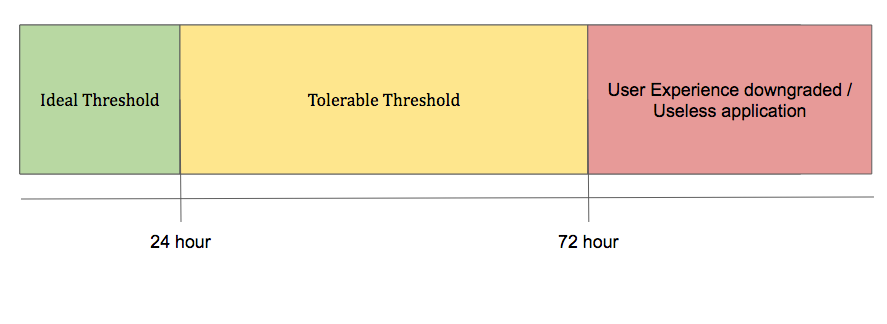
\includegraphics[width=120mm]{Imagens/thresholds.png}
\caption{SLA Thresholds - 3x SLA Delta. \label{fig:thresholds}}
\end{figure}


\subsection{Define \textbf{\textit{database-centered-SLAs}}}

On a Multitier Architecture, databases are generally the last layer to be reached on a user operation. Several other steps are necessary to process a user request, as field validations, security filters and business logic.

From the user-centered SLAs defined on the previous step, another set of SLAs should be proposed on this step, now on database level. These SLAs are called \textbf{\textit{database-centered-SLAs}} in our guidelines and are proposed from the \textbf{\textit{user-centered SLAs}}.

By definition, \textbf{\textit{database-centered-SLAs}} should be ``harder'' than the user-centered SLAs, as other operations are needed in the process of processing a user request. A \textbf{\textit{database-centered SLA}} specifies the Quality-of-Service (QOS) that is expected from the database service while processing an operation.

\textbf{ \textit{Database-centered-SLAs}} should only be defined for the operations that perform transactions at database-level. The same concepts that were defined for \textbf{\textit{user-centered SLAs}} \textbf{\textit{(Ideal Threshold, Tolerable Threshold and SLA Delta)}} are valid for \textbf{\textit{database-centered SLAs}}.

An example of \textbf{\textit{database-centered SLA}} is given for the operations that were enumerated on the the previous step: 

\begin{itemize}
\item{ 
\textbf{Store credit card transaction on my Data Warehouse \textit{(process consumer purchase)}}
\subitem{\textbf{Ideal Threshold:} up to 0.2 seconds;}
\subitem{\textbf{Tolerable threshold:} up to 8 seconds;}
\subitem{\textbf{SLA Delta:} 4.000\% (40x)}
}

\item{
\textbf{Retrieve and perform aggregation operations on selected records \textit{( export summarized report of transactions that happened last week)}}
\subitem{\textbf{Ideal Threshold:} up to 10 hours;}
\subitem{\textbf{Tolerable threshold:} up to 20 hours;}
\subitem{\textbf{SLA Delta:} 200\% (2x)}
}
\end{itemize}

\subsection{Build database-level SLA log alerts}

After defining \textbf{\textit{user-centered}} and \textbf{\textit{database-centered SLAs}}, application architects must define a rate of requests that can be executed on the tolerable-threshold level for each operation.

This \textbf{\textit{rate of faulty requests (ROFR)}} is necessary to avoid unnecessary alerts caused by infrastructural instability, inherently present on cloud providers, as Figure~\ref{fig:sla-agreement} presents.

\subsubsection{Defining a Rate of Faulty Requests (ROFR)}



The \textbf{\textit{rate of faulty requests}} is used in our guidelines to alert application developers that some operations are not being executed with the desired QOS.

\textbf{With a defined \textbf{\textit{ROFR}}, it is possible to build a log / application analyzer that will track if any database operations are breaking the tolerable threshold, or if the rate of faulty requests is above expected.}

If the \textbf{\textit{ROFR}} exceeds the expected level or if a request exceeds the tolerable threshold, an alert should be sent to the Database administrators and maintainers of the application, indicating that an SLA violation was found and that further analysis is needed. This alert can be sent using regular alerting systems, as Email, SMS and push notifications.

Log analyzers and alerts can be implemented within the source code of the application or using external services, such as New Relic, Papertrail and Logstash. 

Once an alert is sent, it should contain \textbf{the timestamp of the moment when the SLA violation was detected} and the process list of what was being executed on database-level at this time. 

It is possible to define a rate of faulty requests for the examples given above: 
\begin{itemize}
\item{ 
\textbf{Store credit card transaction on my Data Warehouse}
\subitem{\textbf{Ideal Threshold:} up to 0.2 seconds;}
\subitem{\textbf{Tolerable threshold:} up to 8 seconds;}
\subitem{\textbf{SLA Delta:} 4.000\% (40x)}
\subitem{\textbf{ROFR: } 10\%}
}

\item{
\textbf{Retrieve and perform aggregation operations on selected records}
\subitem{\textbf{Ideal Threshold:} up to 10 hours;}
\subitem{\textbf{Tolerable threshold:} up to 20 hours;}
\subitem{\textbf{SLA Delta:} 200\% (2x)}
\subitem{\textbf{ROFR:} 30\%}
}
\end{itemize}

In other words, if more than 10\% of the ``Store credit card transactions on my Warehouse'' are performed on a \textbf{Tolerable threshold} level, an alert is fired. If any transaction of this kind lasts more than 8 seconds, another alert is also fired. 

In the second case, if up to 30\% of the transactions are processed within the tolerable threshold, no alert is fired. If any transaction lasts more than 20 hours to be executed, one alert is fired.


\subsection {Verify SLA violation}

When an SLA violation alert is received, it is necessary to know what caused it.

Failures might be possible at machine-level or on the infrastructure that hosts the database server. Hardware issues, network problems and cyber attacks are some factors that may downgrade database performance.  

Extensive and detailed work from application developers might be needed to detect the real cause behind an SLA violation, and the source of each violation is very singular for each application.

Another possible point of failure is the application itself. The mean number of operations per second may have increased, resulting in a downgraded performance of the database; A new feature might be demanding more DB resources and bugs might end up performing faulty requests on the database.

\subsubsection{Further Analysis}
SLA violation alerts contain the exact timestamp of when the violation ocurred, as well as the database process list that was active on the moment of the violation. 

Popular relational databases, as MySQL, Oracle and Postgresql implement a feature called \textit{point-in-time recovery} \cite{pitrmysql} \cite{pitroracle} \cite{pitrposgres}. This feature allows a DB to be dumped and restored to a specific point in time.

As the alert contains the timestamp of when the SLA violation was triggered, it is possible to clone the relational database and restore it to the exact time before the SLA violation was triggered. In this cloned environment it is possible to investigate in detail what caused the SLA Violation. 

If everything is working properly (no issues were found on the database server and on the application), two actions are possible: relax SLA thresholds or propose changes on the current DB Architecture;

\subsection{Propose architectural changes on database-level} 

Not always it is necessary to replace the database to address a performance problem. SQL tunning, denormalizing tables and creating indexes are some ways to improve the performance of applications that use relational databases.

Another option to address performance problems on relational databases would be to scale-up the current DB, buying more powerful hardware. This scenario is not covered by this work, as budget is always a finite resource on companies.

If the SLA remains broken after the architectural changes have been performed on the current DB infrastructure, a NoSQL strategy might be recommended. In this case, a new Database Model (Graph DBs, Document Stores, Key-value stores, etc.) and technology (Neo4j, MongoDB, Couchbase) might be chosen.

Several works, as \cite{6106531} and \cite{5410700} present overviews of NoSQL databases. A good starting point to choose which category of NoSQL Database is the best fit for an application is the CAP theorem \cite{nosqlthoughtworks}, presented on Figure~\ref{fig:cap}. 

\begin{figure}[ht!]
\centering
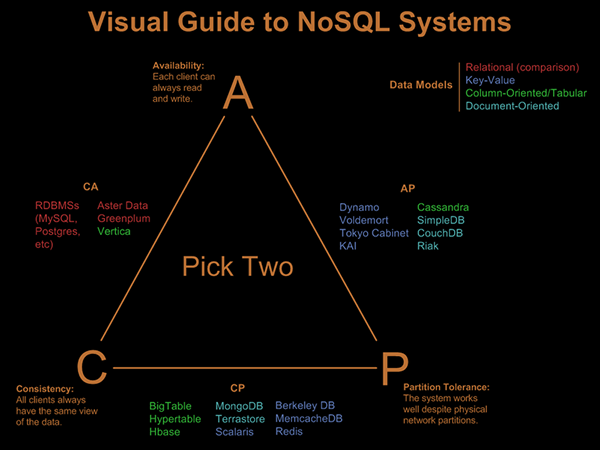
\includegraphics[width=120mm]{Imagens/cap.png}
\caption{CAP Theorem.\cite{captheorem}\label{fig:cap}}
\end{figure}

The CAP Theorem states that that it is possible to have two from the three capabilities in a database: 
\begin{itemize}
\item{Consistency (all nodes see the same data at any point of time);}
\item{Availability (a guarantee that every request receives a response about whether it was successful or failed)}
\item{Partition tolerance (the system continues to operate despite arbitrary message loss or failure of part of the system)
}
\end{itemize}

Relational databases have consistency and availability, resulting in a scale up strategy, presented on Figure~\ref{fig:scaleupout}.

\subsection{Map current schema \& data on the proposed DB architecture}
After choosing the new NoSQL database, it is necessary to map the table's rows and relationships into the concepts of the chosen NoSQL technology. Despite the fact that some NoSQL DBs are schemaless, defining a schema and building indexes help to leverage the perfomance of NoSQL DBs.

To compare the performance of RDBMS vs NoSQL on a specific scenario, the same data should be present on both databases. A Dump \& Restore procedure should be done at this point. i.e: The data should be dumped from the RDBMS and imported on the proposed NoSQL architecture.

The process of mapping (part of) the relational database entities into the new NoSQL schema is very unique to each application and the chosen NoSQL technology. This is a wide topic and not a subject of this work. \cite{bahl2014mysql} shows, for example, how the models of an application might be mapped between different relational \& NoSQL technologies.

Once the new DB architecture is restored with the production data, it is possible to compare the results of the proposed architecture and the old architecture, which is done on the next step.

Over the last sections we have defined thresholds for a Business Intelligence application example. If this application relies on relational databases, it should have several entities, as users, products and commercial transactions. Each of these entities have their own tables, and tables are connected from relationships. 

On a NoSQL strategy, all these entities and relationships could be combined on a single JSON document, as presented on listing~\ref{commercialtransaction}. 

\begin{lstlisting}[language=json,firstnumber=1, caption=BI application commercial transaction represented as a single document., label=commercialtransaction]
{
"id": 12089367123
"user": 12908376123,
"items": [{"id": 01,"category":"food","name":"rice"}, {"id": 21,"category":"drinks","name":"soda"}]
}
\end{lstlisting}
\subsection{Process all DB operations from a historical point}

In this step it is possible to compare the performance of the relational database and the proposed NoSQL architecture. From this point, the following elements should exist as outcomes from the previous steps: 

\begin{itemize}
\item{A production relational database;}
\item{A clone from relational database;}
\item{The proposed NoSQL technology \& data model;}
\item{The same data should be available on the cloned database and on the proposed NoSQL database;}
\item{Logs of the relational database;}
\item{One or more SLA violations;}
\end{itemize}

In a scenario where the relational database will be completely replaced by a NoSQL alternative, it should be possible to execute the same operations on the relational DB and on the proposed NoSQL alternative in any given point in time.

Some DB transitioning processes, however, are performed using a \textit{polyglot persistance} strategy, where an application has several databases. In this case, only some of the application entities will be present on the NoSQL model, and the application data layer will be composed by two or more databases. In this case, only a subset of operations can be executed on the NoSQL side.

A question that may arise at this point is ``What should be the starting-point to compare requests between the relational and NoSQL databases looking for SLA violations?" 

The most complete strategy would be to restore relational database to the oldest point in time where the logs enable and to perform all operations from that point to the point where the SLA violation was triggered. By doing so, it is possible to eventually discover SLA violations that do not exist in the relational architecture and that may arise on the NoSQL architecture.

There are some cases, however, where the volume of data transactions is too large to go back to the oldest point in history. In this cases, a good strategy could be to retrieve all processes that were executing immediately before the SLA violation was fired and go to the point in time when the first of this processes started. 

From the examples given on the previous sections, an alarm would be triggered when the database lasts more than 20 hours to generate a report. When this situation happens, the admins should check the meaningful operations that were running immediately before the alarm is triggered and start to execute the requests in a chronological sequence. 

\subsection{Transitioning Recommendations}

If the proposed NoSQL architecture is able to handle production operations without triggering SLA violations, this is a good sign that the NoSQL might be able to handle the production load.

Transitioning a production database is not an easy and straightforward task, however. It is necessary to change the source code of applications, eventually change some tests and some bugs may be arise during the process. 

Software engineers and database dministrators should assess the impacts of changing database entities and build a transition roadmap considering the following steps:

\begin{enumerate}
\item{Choose entities to be transitioned: as stated previously, it is not necessary to change all database entities in once. If SLA violations are being triggered only for some entities, replacing these entities in a NoSQL architecture can solve the problem.}
\item{Change source code, tests and documentation: Changing the database results in changes on the source code of application and eventually changes on tests and documentation. This should be done as a second step in a transition process. }
\item{Parallelize production calls to both databases: A good practice on database transitioning is to run both storage solutions during a period of time. This means that the relational database is still used as a master storage and the NoSQL is used as a secondary storage. Doing so, a production request should be handled in parallel, but the results of the operations on the secondary database are ignored.}
\item{Perform integrity checks and SLA verifications: At this point it is possible to check if the production requests are correctly being handled by the NoSQL DB. No further SLA violations should be fired at this point.}
\item{Change for a small user base: A small user base can be used to make sure that no other issues will arise from the database transition. This users will have the results from the secondary (NoSQL) database as a result.  }
\item{Change for all users: After a small user base is tested and no SLA violations were found, the transition can be performed for all production users. In this point, (part of) the relational database can be deprecated.}

\end{enumerate}

If the engineers decide not to transition the database in once, it is possible to perform these steps in a cycled manner. i.e: it is possible to transition the entities where SLA violations are being intensively fired at first and then perform other transitioning cycles. This way, the negative impacts of a database transition is amortized. 


\section{Work Phases - TODO: Continue from here}

To provide a better understanding of our work, we splitted the research in six main phases:

\begin{table}[!htb]
   \textsf{\caption{Work Phases.}} \label{tab:WorkPhasesTable}
   \centering
   \medskip
      \begin{tabular}{ | p{1cm}| p{2.5cm} | p {10cm} |}
   \hline
   Phase & Title & Description  \\ \hline
   1 & Identification of Case Studies \& SLAs  & On this step we aim to identify examples where a Database transition is needed or recommended in order to satisfy a SLA.
   We will try to work on production-ready and open-source softwares. If the complexity of these projects is too large for our scope, we will design and develop our own scenarios. \\ \hline
   2 & Plan & After the scenarios have been identified, we will propose architectural changes that could satisfy the SLA. These changes will be proposed by literature reviews and survey of industry experts.\\ \hline
   3 & Do & On this step we implement the architecture proposed on the previous step. \\ \hline
   4 & Check & On the check step we will verify if the proposed architecture and implementation satisfies the SLAs identified on the first step. \\ \hline
   5 & Act & Tweaks can be needed on the proposed architecture and implementation if the SLA is still not satisfied by the changes made on the previous step. On the act phase we investigate what else can be done to satisfy the SLA and refine the process defined on step 2. \\ \hline
   6 & Final Results & On the final step we aim to publish the results of our work on relevant database-related conferences and workshops. \\ \hline
   
   \end{tabular}
\end{table}





Each of these phases is composed by a number of steps, described below:
\begin{enumerate}
\item{Phase 1 - Identification of Case Studies \& SLAs }
   \begin{enumerate}
   \item {Step 1.1 - Scenario identification / Implementation: On this step we will search for open source projects and real-world scenarios where a Relational Database bottleneck has been identified. If the scope of these scenarios become too large, we will implement our own scenarios; }
   \item {Step 1.2 - Identification of broken SLAs: We need to identify that the a set a constraints (i.e: execution time of a query) is not being met by the current architecture;}
   \item {Step 1.3 - Implementation of ``runnable SLAs'' : On this step we will implement executable versions of the SLA identified on the previous step. These ``runnable SLAs" will be used to verify that a set of constraints is not being met by the current architecture. }
   \item {Step 1.4 - Execution reports: After an executable SLA has been identified and implemented, execution reports will be consolidated to prove that the constraints of the SLA are being broken by the current architecture of the scenario.}

   \end{enumerate}


\item{Phase 2 - Plan}
   \begin{enumerate}
   \item{Step 2.1 - Literature Review for each scenario: We will evaluate and search for solutions on how each scenario can make use of a NoSQL Database to meet the desired SLA; }
   \item{Step 2.2 - Survey of industry experts: We will survey industry experts on how they would propose a NoSQL architecture to solve the problem described on each scenario. }
   \end{enumerate}

\item{Phase 3 - Do}
   \begin{enumerate}
   \item{Step 3.1 - Planning of changes: We will gather the results from the previous phase and design the changes that will be performed on each scenario;}
   \item{Step 3.2 - Implementation: We will implement the changes identified on the previous step. }
   \end{enumerate}

\item{Phase 4 - Check}
   \begin{enumerate}
   \item {Step 4.1 - New Execution Reports: The same SLAs identified on the first step will be run on the modified scenarios, and execution reports will be consolidated.}
   \item {Step 4.2 - Comparison of Results: The reports extracted on steps 4.1 and 1.4 will be compared to check if the changes made on Phase 3 satisfied the proposed SLA.}
   \end{enumerate}

\item{Phase 5 - Act}
   \begin{enumerate}
   \item{Step 5.1 - Tweaks on the proposed architecture: If the SLA isn't being met yet, new changes might be needed, and on this step we join together the phases 2, 3 and 4 to iterate over the needed changes. }
   \end{enumerate}


\item{Phase 6 - Final Results}
   \begin{enumerate}
   \item{Step 6.1 - Publish the results: We will submit the results of this study to academical conferences to have feedback from the community. }
   \item{Step 6.2 - Write the final results: All the documents produced by our study and a final dissertation will be sent to the Universidade Federal do Rio Grande do Norte (UFRN).}
   \end{enumerate}

\section{Schedule}

A detailed view of the execution flow of our steps can be seen on Figure~\ref{fig:schedule}. 
\begin{figure}[ht!]
\centering
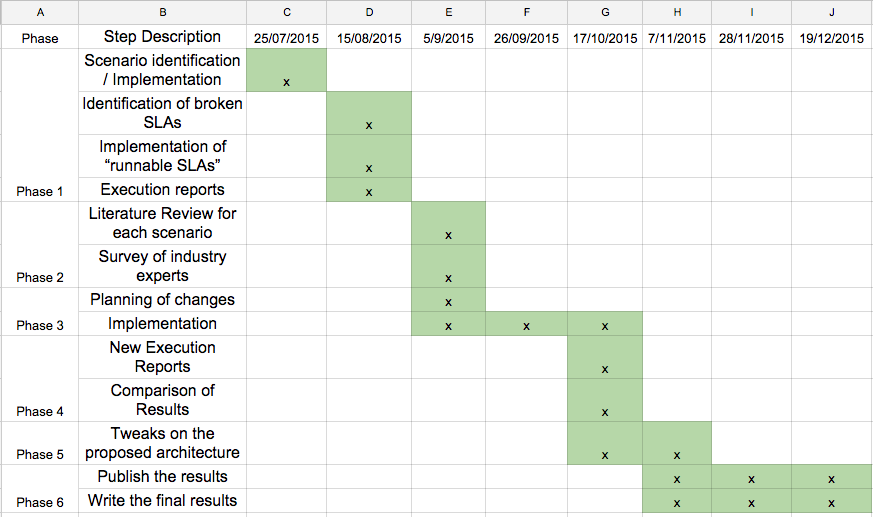
\includegraphics[width=140mm]{schedule.png}
\caption{Schedule.\label{fig:schedule}}
\end{figure}
\end{enumerate}


